\documentclass{beamer}

\input{preamble.tex}
\usepackage{breqn} % Breaks lines

\usepackage{amsmath}
\usepackage{mathtools}

\usepackage{pdfpages} % \includepdf

\usepackage{listings} % R code
\usepackage{verbatim} % verbatim

% Video stuff
\usepackage{media9}

% packages for bibs and cites
\usepackage{natbib}
\usepackage{har2nat}
\newcommand{\possessivecite}[1]{\citeauthor{#1}'s \citeyearpar{#1}}
\usepackage{breakcites}
\usepackage{alltt}

% Setup math operators
\DeclareMathOperator{\E}{E} \DeclareMathOperator{\tr}{tr} \DeclareMathOperator{\se}{se} \DeclareMathOperator{\I}{I} \DeclareMathOperator{\sign}{sign} \DeclareMathOperator{\supp}{supp} \DeclareMathOperator{\plim}{plim}
\DeclareMathOperator*{\dlim}{\mathnormal{d}\mkern2mu-lim}
\newcommand\independent{\protect\mathpalette{\protect\independenT}{\perp}}
   \def\independenT#1#2{\mathrel{\rlap{$#1#2$}\mkern2mu{#1#2}}}
\newcommand*\colvec[1]{\begin{pmatrix}#1\end{pmatrix}}

\newcommand{\myurlshort}[2]{\href{#1}{\textcolor{gray}{\textsf{#2}}}}


\begin{document}

\imageframe{./lecture_includes/mixtape_did_cover.png}


% ---- Content ----

\section{Designing Diff-in-Diff with a Checklist}


\begin{frame}{Different Kinds of Biased Studies}

\begin{itemize}
\item Malfeasance (e.g., data fabrication) and p-hacking have probably grown because of the high returns to top publications
\item Publication bias.  Journals may have preferences for certain results, certain people, or certain thresholds (e.g., $p$-value$<0.05$)
\item Ignorance, low quality data, poor understanding of and therefore misuse of econometric methods
\item But there's a more innocent one that I'll call non-standard errors
\end{itemize}

\end{frame}


\begin{frame}{Non-Standard Errors}

\begin{figure}
    \centering
    \includegraphics[height=0.9\textheight]{./lecture_includes/nick_design}
\end{figure}

\end{frame}

 
\begin{frame}{Non-Standard Errors}
 
\begin{figure}
    \centering
    \includegraphics[height=0.9\textheight]{./lecture_includes/nonstandard_errors2}
\end{figure}

\end{frame}


\begin{frame}{Non-Standard Errors}
 
\begin{figure}
    \centering
    \includegraphics[height=0.9\textheight]{./lecture_includes/borjas_design}
\end{figure}

\end{frame}







\begin{frame}{Controlled Randomization}

\begin{itemize}
\item Randomized controlled trials (RCTs) are not the only design to exploit "coin flips", but the difference is they \textbf{control} the randomization 
\item But not all RCTs are the same -- some control the study extraordinarily well, some can be done so poorly that we learn nothing
\item Quasi-experimental controlled design (QCD) cannot control the randomization, but they can control the design of the study so as to mimic the RCT

\end{itemize}

\end{frame}

	 



\begin{frame}{QCD Needs More "Design Time}

\begin{itemize}
\item Think of an RCT as producing something, but what and how?
\item Well designed RCTs produce \textbf{warranted beliefs} inside humans' minds
\item Imagine then that producing warranted beliefs is a function of "well spent time" designing a study
\end{itemize}

\end{frame}


\begin{frame}{Quasi-Experimental Controlled Design (QCD)}
 
\begin{figure}
    \centering
    \includegraphics[width=\textwidth]{./lecture_includes/qcd}
\end{figure}

\end{frame}









\begin{frame}{Current Practices}
 
\begin{figure}
    \centering
    \includegraphics[width=\textwidth]{./lecture_includes/design_stage}
\end{figure}

\end{frame}


\begin{frame}{How Checklists Saved Lives in Medicine}
    \textbf{Key Idea:} Checklists reduce errors and improve patient safety by standardizing procedures and preventing overlooked steps.

    \begin{itemize}
        \item 
        \textbf{Example:} The WHO Surgical Safety Checklist reduced complications and mortality in surgeries worldwide. A study found a 36\% reduction in major surgical complications.
        \item 
        \textbf{Book:} \textit{The Checklist Manifesto} by Atul Gawande explores how checklists improve outcomes in medicine, aviation, and other fields.
        \item 
        \textbf{Mechanism:} Checklists work by:
        \begin{itemize}
            \item Ensuring critical steps are not missed.
            \item Encouraging teamwork and communication.
            \item Creating a structured, repeatable process for complex tasks.
        \end{itemize}
    \end{itemize}


\end{frame}







\begin{frame}{Why do Diff-in-Diff}

\begin{itemize}
\item Appeal of diff-in-diff has been its simplicity, its transparency, and its ease of conveying analysis to an audience 
	\begin{itemize}
	\item Orley Ashenfelter used it in the 1970s to explain regressions with fixed effects to Bureaucrats in DC 
	\end{itemize}
\item Diff-in-diff is four averages and three subtractions and everyone knows what those are
$$\widehat{\textcolor{blue}{\delta}} = \bigg ( \overline{y}_k^{post(k)} - \overline{y}_k^{pre(k)} \bigg ) - \bigg ( \overline{y}_U^{post(k)} - \overline{y}_U^{pre(k)} \bigg ) $$
\item But $\widehat{\delta}$ is just the OLS coefficient in this regression:
$$Y_{ist} = \alpha_0 + \alpha_1 Treat_{is} + \alpha_2 Post_{t} + \textcolor{blue}{\delta} (Treat_{is} \times Post_t) + \varepsilon_{ist} $$
\end{itemize}

\end{frame}

\begin{frame}{Core assumptions}
\begin{itemize}
\item It can be estimated with a simple regression and has only a few assumptions:
	\begin{enumerate}
	\item SUTVA -- no interference between units
	\item No anticipation -- make sure the baseline (pre period) is not treated (common sense)
	\item Parallel Trends -- Models the missing potential outcome, $Y^0$ and \textbf{is not testable}
	\end{enumerate}
\item Parallel trends is a strong assumption -- it is equivalent to assuming away problem and our best tests are just falsifications
\end{itemize}

\end{frame}






\subsection{Step 1: Choosing Target Parameter}

\begin{frame}{Step 1: Choosing Target Parameter (Concealed Carry Example)}

\begin{itemize}
\item Lott and Mustard (1997) found that concealed carry gun laws \textbf{reduced murders} using county-level data 1977-1992
\item Subsequent analysis by John Donohue and others would criticize the study on several grounds
	\begin{itemize}
	\item County-level data had problems due to flawed imputation by the FBI
	\item Lack of robustness -- results differed when using state-level data
	\end{itemize}
\item Causal parameters are \emph{averaged treatment effects} and that has two elements
	\begin{itemize}
	\item What population's treatment effects are you averaging
	\item What weight are you using to do that averaging?
	\end{itemize}
\end{itemize}

\end{frame}

\begin{frame}{Average Treatment Effects}

\begin{figure}
    \centering
    \includegraphics[width=\textwidth]{./lecture_includes/step1_table}
\end{figure}

$ATE =  \frac{1-1+0+0+1+1}{6} = 0.33$

\end{frame}

\begin{frame}{Average Treatment Effects}

\begin{figure}
    \centering
    \includegraphics[height=0.8\textheight]{./lecture_includes/step1_y1y0}
\end{figure}


\end{frame}

\begin{frame}{Average Treatment Effect on the Treated}

\begin{figure}
    \centering
    \includegraphics[height=0.8\textheight]{./lecture_includes/step1_att}
\end{figure}


\end{frame}


\begin{frame}{Different Levels of Aggregation, Different Weights}

\begin{figure}
    \centering
    \includegraphics[height=0.8\textheight]{./lecture_includes/step1_weighted}
\end{figure}


\end{frame}

\begin{frame}{Different Levels of Aggregation, Different Weights}


\begin{itemize}
\item Heterogenous treatment effects is causing this, but so is weighting
\item Consider Texas
	\begin{itemize}
	\item Texas has 31 million residents
	\item Texas 254 counties
	\end{itemize}
\item Where do they live?
	\begin{itemize}
	\item 13 million live in Harris, Dallas, Fort Worth, San Antonio and Austin, or rather 41\% 
	\end{itemize}
\item What if concealed carry increases firearm deaths in cities, but reduces them in counties, because of sorting by treatment effects?
\end{itemize}

\end{frame}

\begin{frame}{Simulation}

\begin{itemize}
\item Assume a state with 30 million people and 254 counties
	\begin{itemize}
	\item 15 million live in 5 counties
	\item 15 million live equally spread in the other 249 counties (around 60,000 each)
	\end{itemize}
\item Average treatment effect in top 5 counties for concealed carry is +5 each county
\item Average treatment effect in all other 249 counties is is -1 each county
\item ATE for the state is positive, but ATE for the counties is negative, and \textbf{both are right}
\end{itemize}

\end{frame}



\begin{frame}{Different Levels of Aggregation, Different Weights}

\begin{figure}
    \centering
    \includegraphics[height=0.7\textheight]{./lecture_includes/step1_moreate}
\end{figure}

\end{frame}



\begin{frame}{You must own your choices}

\begin{itemize}
\item Diff-in-diff identifies the ATT, but it's still a weighted average over the treated units \emph{in your sample}
\item Do you want to know the ATT for the \emph{average person} or the \emph{average county}?
	\begin{itemize}
	\item It depends if your study is about counties or people
	\item Maybe there is a legitimate reason to study counties -- they are distinct communities and maybe they want to govern themselves
	\item You can always use population weights but why?  What parameter are you trying to weight towards?
	\end{itemize}
\item Since you're averaging over \emph{units} in \emph{data}, it's imperative you make a decision early on as it changes what you decide
\end{itemize}

\end{frame}


\subsection{Step 2: Is Everyone Treated at the Same Time?}

\begin{frame}{Step 2: Is Everyone Treated at the Same Time?}

\begin{itemize}
\item Cohorts and groups words used interchangeably in diff-in-diff
\item Cohorts describe \emph{when} units were treated at the same time
\item Count those units and show them in a table so that we can see who is in each cohort, how large they are, and when this happened
\item Include the "already treated" and the "never treated" in your counts if they exist
\end{itemize}

\end{frame}

\begin{frame}

\begin{figure}
    \centering
    \includegraphics[height=0.9\textheight]{./lecture_includes/treated_at_same_time}
\end{figure}

\end{frame}



\subsection{Step 3: Plot Treatment Rollout}


\begin{frame}{Step 3: Plot Treatment Rollout}

\begin{figure}
    \centering
    \includegraphics[height=0.95\textheight]{./lecture_includes/step3_panelview}
\end{figure}

\end{frame}




\subsection{Step 4: Is Unconditional Parallel Trends Plausible?}

\begin{frame}{Step 4: Is Unconditional Parallel Trends Plausible?}

\begin{itemize}
\item Two units would have evolved similar over time had neither been treated:
	$$\textcolor{red}{\Delta E[Y^0|D=1]} = \Delta E[Y^0|D=0]$$
\item It is not testable, but let's consider an example from a different study of mine
\item Me, Christine Durrance and Melanie Guldi are studying online dating's effects on birth rates using Craigslist's "personals" section which rolled out from 2000 to 2010 to different markets
\item County level birth rates without any controls versus controlling for one variable -- a 9-digit variable (RUCC) measuring how urban that county is
\end{itemize}

\end{frame}


\begin{frame}

\begin{figure}
    \centering
    \includegraphics[height=0.95\textheight]{./lecture_includes/es_br1544_combined.png}
\end{figure}

\end{frame}

\begin{frame}{What the heck}

\begin{itemize}
\item What happened?  Craigslist tended to target urban counties so treatment were highly urban and control highly rural
\item Remember that what's missing in the ATT is $\textcolor{red}{E[Y^0|D=1]}$ and we use the control group trends in its $Y^0$ to \emph{impute} the missing $\textcolor{red}{E[Y^0|D=1]}$
\item It's actually pretty basic -- do you think cities have different birth rate trends than counties?  If so, then that imputation is likely to be bad
\item But what if you imputed $Y^0$ apples for apples -- use cities in the control to impute cities in the treatment

\end{itemize}
\end{frame}


\begin{frame}{You may need to replace PT}

\begin{itemize}
\item Two parallel trends assumptions
	\begin{enumerate}
\item Unconditional parallel trends: means parallel trends holds for treatment and control
\item Conditional parallel trends: means only units that are similar on covariates would have evolved similarly
	\end{enumerate}
\item Covariates in diff-in-diff aren't really "omitted variable bias" so much as they are designed to fix broken parallel trends
\item Kahn-Lang and Lang (XXX) say that if your two groups are pretty different at baseline on outcomes, while it does not violate PT, it might and definitely means treatment was not random
\end{itemize}

\end{frame}

\begin{frame}{}

\begin{figure}
    \centering
    \includegraphics[height=0.30\textheight]{./lecture_includes/selection_pt}
\end{figure}

You're fine if and only if units select into treatment based on:
\begin{enumerate}
\item Constant trends for every unit 
\item Selection on fixed effects 
\item Selection on baseline $Y^0$ 
\item Selection on $\Delta E[Y^0]$ -- technically you're fine, but it will screw up your event studies
\item Selection on covariates  -- you'll need to control for them
\item And some other technical stuff (e.g., Martingale process)
\end{enumerate}

\end{frame}


\begin{frame}{Assume Conditional PT}

\begin{figure}[h!]
    \centering
    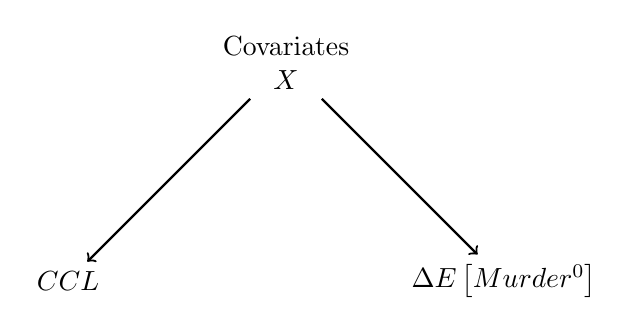
\begin{tikzpicture}[
        node distance=2.5cm,
        every node/.style={align=center},
        line/.style={->, thick},
    ]
    % Nodes
    \node (X) {Covariates \\ \( X \)};
    \node (D) [below left of=X, xshift=-1cm, yshift=-1cm] {\( CCL \)};
    \node (DeltaY0) [below right of=X, xshift=1cm, yshift=-1cm] {\( \Delta E\left[Murder^0\right] \)};
    % Arrows
    \draw[line] (X) -- (DeltaY0);
    \draw[line] (X) -- (D);
    \end{tikzpicture}
\caption{DAG representing differences in county-level covariate composition (\(X\)) across treatment and control groups (\(D\)) and their determination of the untreated potential \emph{murder rate} trends (\(\Delta E\left[Murder^0\right]\)).}
\label{fig:covariates_pathway1}
\end{figure}

\end{frame}

\begin{frame}{Picking covariates}

\begin{itemize}
\item You're missing $Y^0$ -- so ask yourself, "what are the ordinary determinants of county-level murder during this period of time?"
\item 1977 to 1992
	\begin{itemize}
	\item Drugs (crack cocaine)
	\item Cities had different homicide rates than rural counties
	\item Police, incarceration
	\item Demographics (e.g., race shares, age shares) and economic things (e.g., poverty, per capital income, AFDC rolls)
	\item Maybe throw it all into LASSO using only the $Y^0$ values (maybe pre-treatment murders)
	\end{itemize}
\item That's the $X \rightarrow Y^0$ part -- become an expert on your left-hand-side variable for this period of time 
\item But just because some $X \rightarrow Y^0$ does not mean you have to control for it -- only if the two groups are \emph{imbalanced}
\end{itemize}

\end{frame}

\subsection{Step 5: Pick Your Control Group}

\begin{frame}{Step 5: Pick Your Control Group}

\begin{itemize}

\item One of the sins created by OLS was the ability to throw the kitchen sink into one model and never know who was being compared to who
	\begin{itemize}
	\item Causal inference is hard and easy -- don't confuse the hard with the easy
	\item If you can't say who the comparison group is, start there because it should be you choosing it, not the model
	\end{itemize}
\item These are simple comparisons -- who do you want to be the comparison group?
\item For instance, do you want to compare treated units with never treated units?
	\begin{itemize}
	\item Weird that they never got treated though right?
	\end{itemize}
\item Or do you want to compare with not-yet-treated?  Share anecdote about driver license law and undocumented workers
\end{itemize}

\end{frame}

\subsection{Step 6: Check Covariate Imbalance}

\begin{frame}{Step 6: Check Covariate Imbalance}

\begin{itemize}
\item You think you want to appeal to conditional parallel trends and you have chosen your covariates -- now what?
\item Next step is the $X \rightarrow D$ part of that DAG
\item When you have selection on covariates, then it automatically means that the treatment group and control group have different distributions of $X$, so check the balance
\end{itemize}

\end{frame}


\begin{frame}
    \frametitle{Baseline Covariates and Normalized Difference}
    \begin{itemize}
        \item Baseline covariates are measured before treatment ($t-1$). Check for balance between treatment and control groups.
        \item Report the averages of covariates for both groups in a table.
        \item The normalized difference is calculated as:
        $$ \text{Norm. Diff}_\omega = \frac{\overline{X}_{\omega,T} - \overline{X}_{\omega,C}}{\sqrt{(S_{\omega,T}^2 + S_{\omega,C}^2)/2}} $$
        \item The normalized difference measures imbalance; it should be less than 0.25 to avoid problematic imbalance Imbens and Rubin (2015).
    \end{itemize}
\end{frame}


\begin{frame}{}

\begin{figure}
    \centering
    \includegraphics[height=0.80\textheight]{./lecture_includes/step6_imbalance}
\end{figure}

\end{frame}



\subsection{Step 7: Plot Average Outcomes Across Cohorts}

\begin{frame}{Step 7: Plot Average Outcomes Across Cohorts}

\begin{itemize}
\item We are literally \textbf{seven} steps into the checklist and this is the first time we are looking at the outcomes (except for baseline)
\item You want to avoid "peeking" at the outcome because you're not wanting to bias yourself and you want this to mimic the RCT as best as you can
\item This is another reason I get frustrated with TWFE -- you can't separate the design from the estimation because the left-hand-side and right-hand-side are both there 
\item Plot the evolution of the mean homicides over time \emph{for each cohort}
\end{itemize}

\end{frame}

\begin{frame}

\begin{figure}
    \centering
    \includegraphics[height=0.85\textheight]{./lecture_includes/step7_outcomes}
\end{figure}

\end{frame}






\subsection{Step 8: Estimator Selection and Assumptions}

\begin{frame}{Step 8: Estimator Selection and Assumptions}

\begin{itemize}
\item Some options with simple diff-in-diff
	\begin{enumerate}
	\item TWFE with or without covariates (you'll need additional assumptions for TWFE with controls)
	\item Regression adjustment (Heckman, Ichimura and Todd 1997), inverse probability weighting (Abadie 2005) or double robust (Sant'Anna and Zhou 2020)
	\item Double debiased machine learning (Chang 2020)
	\end{enumerate}
\item Think of there being two options with differential timing 
	\begin{enumerate}
	\item Aggregating ATT(g,t) using Callaway and Sant'Anna or Sun and Abraham
	\item Imputation using Borusyak, Jaravel and Speiss, or Wooldridge
	\end{enumerate}
\item Which one do you want? 
\end{itemize}

\end{frame}

\begin{frame}{Comparing them}

\begin{itemize}
\item Aggregating group-time ATT(g,t)
	\begin{itemize}
	\item CS and SA have the most flexible parallel trends assumption
	\item CS imposes no homogeneity restrictions with respect to covariates
	\item CS estimates a propensity score or nonparametric outcome regression to handle covariates so if you have poor overlap, it'll be biased even with conditional PT
	\end{itemize}
\item Imputation
	\begin{itemize}
	\item BJS is efficient with spherical errors (fat chance)
	\item BJS and Wooldridge require PT to hold in all pre-treatment periods which gives more power
	\item But don't need overlap as they impute using estimated fixed effects and extrapolation
	\end{itemize}
\item Probably those are the guide -- let it be because you feel more comfortable with the assumptions
\end{itemize}
\end{frame}

\subsection{Step 9: Checking for Parallel Trends Violations with Falsifications, Event Studies and Sensitivity Analysis}

\begin{frame}{Step 9: Falsification, Event Studies and Sensitivity Analysis}

\begin{itemize}
\item Causal inference is about \emph{warranted beliefs} -- should you or should you not believe the \emph{causal claim}?
\item Your DiD \emph{results} are like the claim of guilt, but your DiD results are \emph{not} the smoking gun
	\begin{itemize}
	\item Your table of regression coefficients \emph{is not enough} for evidence
	\item You need to do more to provide a justification for parallel trends
	\end{itemize}
\item You need to provide evidence for parallel trends against several well known vulnerabilities
\item Evidence will be bite, falsifications, mechanisms and event study data visualization 
\item We will mix the parallel trends violations with the evidence concept before getting into advanced estimators
\end{itemize}

\end{frame}


\begin{frame}{Court metaphor}

	\begin{itemize}
	\item Think of yourself as a prosecutor arguing against a defense attorney to convince a judge and jury of a defendant's guilt
	\item The claim the defendant is guilty is your table of main results
	\item But the claim is not the evidence -- you have to back up that claim 
	\item Your evidence of guilt is the smoking gun, the fingerprints, the eye witnesses, the footprints in the mud outside the house
	\item If your claim is supported by weak evidence, then no one \emph{should} convict -- it would be borderline corruption if they did 
	\end{itemize}

\end{frame}


\begin{frame}{Medicaid and Affordable Care Act example}

\begin{figure}
\includegraphics[scale=0.25]{./lecture_includes/medicaid_qje}
\end{figure}

\end{frame}
\begin{frame}{Their Evidence versus Their Result}

\begin{itemize}
\item \textbf{Bite} -- they will show that the expansion shifted people into Medicaid and out of uninsured status
\item \textcolor{black}{\textbf{Placebos}} -- they show that there's no effect of Medicaid on a similar group that didn't enroll
\item \textbf{Event study} -- they will lean hard on those dynamic plots
\item \textcolor{red}{\textbf{Main results}} -- with all of this, they will show Medicaid expansion caused near elderly mortality to fall
\item \textcolor{black}{\textbf{Mechanisms}} -- they think they can show it's coming from people treating diseases causing mortality declines to compound over time
\end{itemize}

\end{frame}

\begin{frame}{Bite}

\begin{itemize}
\item Bite is a labor economist's phrase, often used with the minimum wage, to say that the minimum wage actually was binding in the first place
\item Here it means when US states made Medicaid more generous, people got on Medicaid who would not have been on it otherwise
\item And as a bonus, would not have been insured at all without it
\item Not the most exciting result, but imagine if the main results on mortality were shown but there was no evidence for bite -- is it believable?
\end{itemize}

\end{frame}

\begin{frame}{Eligibility}

	\begin{figure}
\includegraphics[scale=0.425]{./lecture_includes/Miller_Medicaid1.png}
	\end{figure}

\end{frame}

\begin{frame}{Enrollment}

	\begin{figure}
\includegraphics[scale=0.425]{./lecture_includes/Miller_Medicaid2.png}
	\end{figure}

\end{frame}

\begin{frame}{Uninsured}

	\begin{figure}
\includegraphics[scale=0.425]{./lecture_includes/Miller_Medicaid3.png}
	\end{figure}

\end{frame}




\begin{frame}{Falsification}

\begin{itemize}

\item Their study focuses on ``near elderly'', which means just under 65
\item They choose just under 65 because in the US, 65 and older are eligible for Medicare so more generous Medicaid is irrelevant
\item \emph{But} probably the near elderly and the elderly are equally susceptible to unobserved factors correlated with the treatment
\item So they painstakingly examine the effects on elderly as a falsification as this will strengthen the parallel trends assumption on the near elderly
\end{itemize}

\end{frame}

\begin{frame}{Falsifications on elderly}

	\begin{figure}
\includegraphics[scale=0.425]{./lecture_includes/placebo_medicaid}
	\end{figure}

\end{frame}

\begin{frame}{Main result}

\begin{itemize}

\item Finally they focus on the main result -- and there's more in the paper than I'm showing
\item Event study plots with same specification as the rest allowing us to look at the pre-trends and the post-treatment coefficients
\item If parallel trends holds, then the post-treatment coefficients are interpreted as ATT parameter estimates for each time period
\item The result alone isn't nearly as strong the result in combination with the rest, but it could still be wrong as parallel trends is ultimately not verfiable
\end{itemize}

\end{frame}



\begin{frame}{Near elderly mortality and Medicaid expansion}

	\begin{figure}
	\includegraphics[scale=0.3]{./lecture_includes/Miller_Medicaid4.png}
	\end{figure}

\end{frame}

\begin{frame}{Summarizing evidence and results}

\begin{itemize}
\item \textbf{Bite}: Increases in enrollment and reductions in uninsured support that there is adoption of the treatment
\item \textbf{Event studies}: Compelling graphics showing similarities between treatment and control
\item \textbf{Falsifications}: no effect on a similar group who isn't eligible
\item \textcolor{red}{Main results}: 9.2\% reduction in mortality among the near-elderly
\item \textcolor{red}{Mechanism}: ``The effect is driven by a reduction in disease-related deaths and grows over time.''
\end{itemize}

\end{frame}

\begin{frame}{Sensitivity Analysis}

\begin{itemize}
\item Assume the worst -- use the absolute worst gap in pre-trends and imagine PT broke by that much post-treatment
\item How bad does that have to get before your treatment effect coefficient covers zero?
\item Called \texttt{honestdid} by Rambachan and Roth (2023) 
\item Don't think of it as rejecting PT -- it's just saying how dependent on it you are
\end{itemize}

\end{frame}

\begin{frame}{Sensitivity Analysis}

	\begin{figure}
    \includegraphics[height=0.85\textheight]{./lecture_includes/step9_roth}
	\end{figure}

\end{frame}







\subsection{Step 10: DDDiD, or "Don't Do Diff-in-Diff}


\begin{frame}{Step 10: DDDiD, or "Don't Do Diff-in-Diff}

\begin{itemize}
\item If you simply cannot satisfy yourself that the parallel trends assumption holds because there is no adequate comparison group, or whatever, you have to punt on diff-in-diff
\item But that's okay because the goal was never to use diff-in-diff -- the goal was to get an estimated effect of a parameter you wanted to know that was credible
\item You'll probably end up at step 10 more if you introduce a design stage, but that's not the end of the world, because there's still other panel methods (e.g., synthetic control)


\end{itemize}

\end{frame}

\begin{frame}{Replacing Control With Design Time}

\begin{itemize}
\item We often get distracted by shiny objects:
	\begin{itemize}
	\item If only I was better at programming in advanced languages
	\item If only I knew all of the latest methods in causal inference and econometrics
	\end{itemize}
\item Programming and econometrics without a design stage does not create those warranted beliefs
\end{itemize}

\end{frame}




\begin{frame}{Design Trumps Analysis}

	\begin{figure}
	\includegraphics[scale=0.3]{./lecture_includes/rubin_design_trump}
	\end{figure}

\end{frame}


\begin{frame}{Design Trumps Analysis}

\begin{itemize}

\item Your goal is \emph{credible answers} and it's helpful to have the RCT in your mind for many reasons
\item One reason is that RCT teaches us what works -- randomization
\item But another reason is that \emph{designing} RCTs is independently a gold standard -- those researchers are meticulous, even going so far as to submit their \emph{designs} to a journal before doing the analysis
\item No reason we can't do that -- I did that in Ozler, et al (2021) in \emph{Journal of Development Economics}
\item Key for me has been to love all parts of research, including design, love the scientific methods we have been given, love growing and learning, enjoy the process -- that's really the only part we can control
\end{itemize}

\end{frame}


\begin{frame}{Current Practices}
 
\begin{figure}
    \centering
    \includegraphics[width=\textwidth]{./lecture_includes/design_stage}
\end{figure}

\end{frame}



\end{document}


